
\section{TTS Move} % (fold)
\label{sec:tts_move}

    Il terzo tipo di mossa che si è scelto di implementare consiste nella selezione di tre \emph{tiles} in sequenza, secondo l'asse verticale od orizzontale ( rispettivamente Figure \ref{fig:tts1} e \ref{fig:tts2}). La mossa segue lo stesso principio delle precedenti; in questo senso la selezione delle sequenze (di seguito chiamate anche ``three-tile streak'') viene fatta a priori all'interno dello stato della \emph{board} di gioco. Tale selezione, viene rigenerata nel caso si effettui una \texttt{SelectBest($\cdots$)} (si noti che, altrimenti, chiamate successive di \texttt{SelectBest($\cdots$)}, non porterebbero alcun miglioramento alla configurazione), mentre viene usato un contatore interno allo stato per regolare la vita di una data selezione per l'uso di \texttt{RandomMove($\cdots$)}.

    \begin{figure}[H]
        \centering
        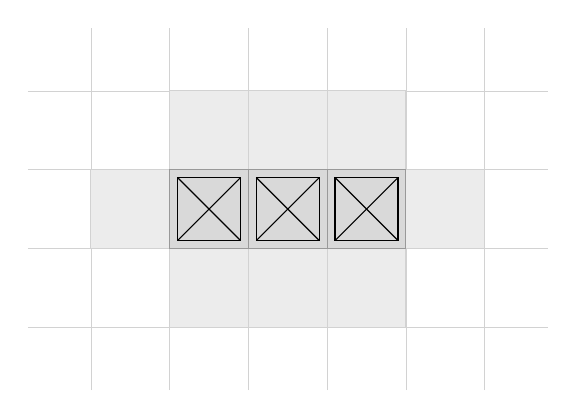
\begin{tikzpicture}
            \draw[step=1cm,gray!35!white,very thin] (.2,.2) grid (6.8,4.8);
            \foreach \x/\y in {2/1,3/1,4/1,1/2,2/3,3/3,4/3,5/2}
                \filldraw[fill=gray!15!white,draw=gray!35!white] (\x,\y) rectangle (\x+1,\y+1);
            \foreach \x/\y in {2/2,3/2,4/2}
            {
                \filldraw[fill=gray!30!white,draw=gray!80!white] (\x,\y) rectangle (\x+1,\y+1);
                \draw[black] (\x+.1,\y+.1) rectangle (\x+.9,\y+.9);
                \draw[black] (\x+.1,\y+.1) -- (\x+.9,\y+.9);
                \draw[black] (\x+.9,\y+.1) -- (\x+.1,\y+.9);
            }
        \end{tikzpicture}
        \caption{Horizontal Three--Tile Streak Selection}
        \label{fig:tts1}
    \end{figure}

    \begin{figure}[H]
        \centering
        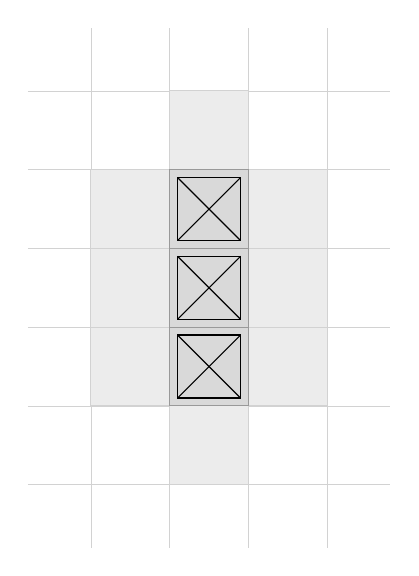
\begin{tikzpicture}
            \draw[step=1cm,gray!35!white,very thin] (.2,.2) grid (4.8,6.8);
            \foreach \x/\y in {2/1,1/2,3/2,1/3,3/3,1/4,3/4,2/5}
                \filldraw[fill=gray!15!white,draw=gray!35!white] (\x,\y) rectangle (\x+1,\y+1);
            \foreach \x/\y in {2/2,2/3,2/4}
            {
                \filldraw[fill=gray!30!white,draw=gray!80!white] (\x,\y) rectangle (\x+1,\y+1);
                \draw[black] (\x+.1,\y+.1) rectangle (\x+.9,\y+.9);
                \draw[black] (\x+.1,\y+.1) -- (\x+.9,\y+.9);
                \draw[black] (\x+.9,\y+.1) -- (\x+.1,\y+.9);
            }
        \end{tikzpicture}
        \caption{Vertical Three--Tile Streak Selection}
        \label{fig:tts2}
    \end{figure}

    La selezione delle \emph{three-tile streaks} è definita con un unico ciclo attraverso la board di gioco. Per ogni coordinata viene stabilito se essa sia coperta da una sequenza, facendo uso di una distribuzione di probabilità \emph{bernoulliana} (simulata con il generatore random con distribuzione uniforme fornito dal framework \emph{EasyLocal++}). Ad ogni nuovo inserimento nella board viene anche fatto un controllo di \emph{feasibility} in modo da evitare inserimenti invalidanti.

    Questo semplice algoritmo di selezione delle sequenze non genera ogni possibile configurazione con uguale probabilità, ma risulta più efficiente di altre soluzioni. Inoltre, modificando in modo opportuno i parametri di generazione delle \emph{streak} è possibile generare selezioni massimali con un'alta probabilità.

    \begin{figure}[H]
        \centering
        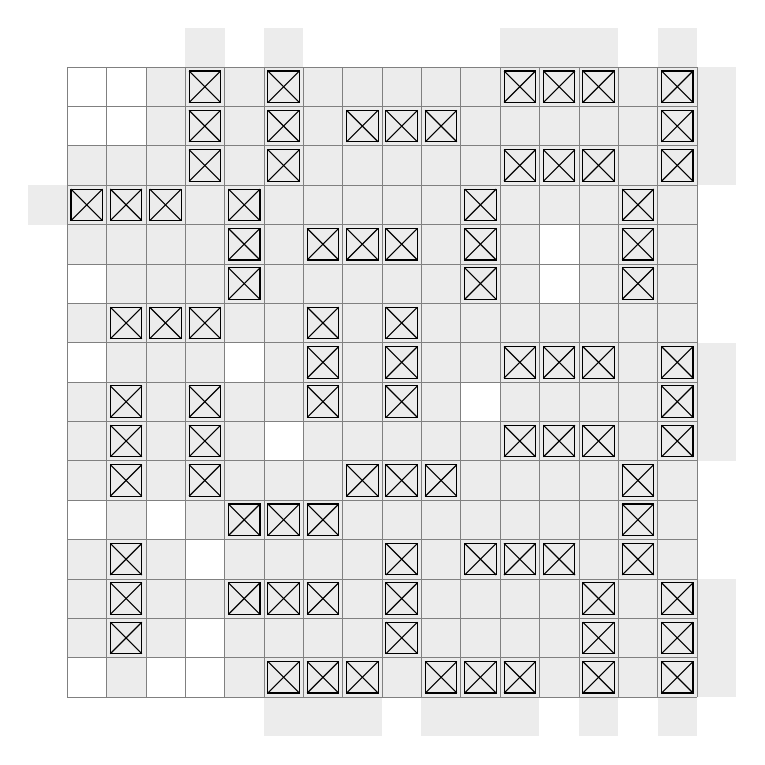
\begin{tikzpicture}
            %\foreach \x/\y in {2/1,1/2,3/2,1/3,3/3,1/4,3/4,2/5}
            %    \filldraw[fill=gray!15!white,draw=gray!35!white] (\x,\y) rectangle (\x+1,\y+1);
            \foreach \x/\y/\r in {.5/1/1,2.5/2/0,4/2.5/0,7/2/1,6.5/.5/1,0.5/3/1,0.5/6/0,3/0/0,2.5/1/0,4/1/1,5.5/1.5/0,5/0/0,7.5/.5/1,3/4/1,6/4/0,1.5/3/1,1/4.5/0,2/5.5/1,1.5/7/1,6/3/0,7.5/3.5/1,4/4/1,3.5/5.5/0,2.5/7/1,4/7/0,5/5.5/1,6/6.5/0,6/7.5/0,7.5/7/1,7/5.5/1}
            {
                \fill[fill=gray!15!white] (\x,\y) rectangle (\x+.5,\y+.5);
                \draw[black] (\x+.05,\y+.05) rectangle (\x+.45,\y+.45);
                \draw[black] (\x+.05,\y+.05) -- (\x+.45,\y+.45);
                \draw[black] (\x+.45,\y+.05) -- (\x+.05,\y+.45);

                \fill[fill=gray!15!white] (\x+.5*\r-.5,\y-.5*\r) rectangle (\x+.5*\r,\y-0.5*\r+.5);
                \draw[black] (\x+.5*\r-.5+.05,\y-.5*\r+.05) rectangle (\x+.5*\r-.05,\y-0.5*\r+.5-.05);
                \draw[black] (\x+.5*\r-.5+.05,\y-.5*\r+.05) -- (\x+.5*\r-.05,\y-0.5*\r+.5-.05);
                \draw[black] (\x+.5*\r-.5+.05,\y-0.5*\r+.5-.05) -- (\x+.5*\r-.05,\y-.5*\r+.05);

                \fill[fill=gray!15!white] (\x-.5*\r+.5,\y+.5*\r) rectangle (\x-.5*\r+.5+.5,\y+.5*\r+.5);
                \draw[black] (\x-.5*\r+.5+.05,\y+.5*\r+.05) rectangle (\x-.5*\r+.5+.5-.05,\y+.5*\r+.5-.05);
                \draw[black] (\x-.5*\r+.5+.05,\y+.5*\r+.05) -- (\x-.5*\r+.5+.5-.05,\y+.5*\r+.5-.05);
                \draw[black] (\x-.5*\r+.5+.5-.05,\y+.5*\r+.05) -- (\x-.5*\r+.5+.05,\y+.5*\r+.5-.05);

                \fill[fill=gray!15!white] (\x-.5*\r,\y+.5*\r-.5) rectangle (\x-.5*\r+.5,\y+.5*\r-.5+.5);
                \fill[fill=gray!15!white] (\x-.5*\r+.5*\r-.5,\y+.5*\r-.5*\r-.5) rectangle (\x+.5*\r-.5-.5*\r+.5,\y-.5*\r+.5*\r-.5+.5);
                \fill[fill=gray!15!white] (\x-.5*\r-.5*\r+.5,\y+.5*\r+.5*\r-.5) rectangle (\x-.5*\r+.5-.5*\r+.5,\y+.5*\r+.5*\r-.5+.5);
                \fill[fill=gray!15!white] (\x+.5*\r,\y-.5*\r+.5) rectangle (\x+.5*\r+.5,\y-.5*\r+.5+.5);
                \fill[fill=gray!15!white] (\x+.5*\r-.5+.5*\r,\y-.5*\r-.5*\r+.5) rectangle (\x+.5*\r-.5+.5*\r+.5,\y-.5*\r-.5*\r+.5+.5);
                \fill[fill=gray!15!white] (\x-.5*\r+.5+.5*\r,\y+.5*\r-.5*\r+.5) rectangle (\x-.5*\r+.5+.5*\r+.5,\y+.5*\r-.5*\r+.5+.5);
                \fill[fill=gray!15!white] (\x+\r-1,\y-\r) rectangle (\x+\r-1+.5,\y-\r+.5);
                \fill[fill=gray!15!white] (\x-\r+1,\y+\r) rectangle (\x-\r+1+.5,\y+\r+.5);
            }
            \draw[step=.5cm,gray,very thin] (0,0) grid (8,8);
        \end{tikzpicture}
        \caption{Example of feasible maximal selection of Three--Tile Streaks}
    \end{figure}

    Una volta determinata la selezione delle \emph{three-tile streaks} si ricerca un loro ricombinamento, secondo la semantica del tipo di mossa selezionata. Il ricombinamento della selezione prevede un ulteriore grado di libertà, dipendente dall'orientamento di una \emph{streak} (Figura \ref{fig:tts4})
    
    \begin{figure}[H]
        \centering
        \begin{tikzpicture}
            \draw[step=1cm,gray!35!white,very thin] (.2,.2) grid (10.8,6.8);
            \foreach \x/\y in {2/1,1/2,3/2,1/3,3/3,1/4,3/4,2/5,6/1,7/1,8/1,6/3,7/3,8/3,6/5,7/5,8/5,5/2,9/2,5/4,9/4}
                \filldraw[fill=gray!15!white,draw=gray!35!white] (\x,\y) rectangle (\x+1,\y+1);
            \foreach \x/\y/\n in {2/2/3,2/3/2,2/4/1,6/2/1,7/2/2,8/2/3,6/4/3,7/4/2,8/4/1}
            {
                \filldraw[fill=gray!30!white,draw=gray!80!white] (\x,\y) rectangle (\x+1,\y+1);
                \draw[black] (\x+.1,\y+.1) rectangle (\x+.9,\y+.9);
                \draw[black] (\x+.1,\y+.1) -- (\x+.9,\y+.9);
                \draw[black] (\x+.9,\y+.1) -- (\x+.1,\y+.9);

                \node[circle,minimum size=.4,color=black,fill=gray!30!white] at (\x+.5,\y+.5) {\n};

            }
            \draw (3.5,4.5) edge[-triangle 90,out=50] (7.5,5.2);
            \begin{scope}[yscale=-1,yshift=-7cm]
                \draw (3.5,4.5) edge[-triangle 90,out=50] (7.5,5.2);
            \end{scope}
        \end{tikzpicture}
        \caption{Streak recombination}
        \label{fig:tts4}
    \end{figure}

    Anche in questo caso, per la \texttt{SelectBest($\cdots$)} viene utilizzato l'algoritmo Ungherese che riduce un problema di ricombinazione delle tessere selezionate come un problema di \emph{maximum matching}.



% section tts_move (end)